
\chapter{ಮುಗಿಲೆತ್ತರದ ಹಿಮಾಲಯ ಅಳೆಯಲು ಹರಸಾಹಸ}

\vskip -5pt

ಉತ್ತರದ ಹಿಮಾಲಯವು ಮಂಜು ಮುಸುಕಿದ ಮುಗಿಲೆತ್ತರವಾದ ಭವ್ಯ ದಿವ್ಯ ಪರ್ವತಗಳಿರುವ ಪ್ರದೇಶ. ಸುಲಭಕ್ಕೆ ತಲುಪಲು ಆಗದ ಅನುಪಮ ಎತ್ತರದ ಪರ್ವತಗಳು ಅವು. ಅವುಗಳ ಸರ್ವೇಯು ಸಹ ಸುಲಭ ಸಾಧ್ಯವಲ್ಲ. ಯಾರಾದರೂ ಅವುಗಳ ಎತ್ತರವನ್ನು ಅಳೆದು ಎತ್ತರ ಇಂತಿಷ್ಟು ಎಂದು ಹೇಳಿದರೆ, ಸುಲಭಕ್ಕೆ ಒಪ್ಪಿ ಸ್ವೀಕರಿಸಲು ಸಾಧ್ಯವಾಗದ ದುರ್ಗಮ ಪರ್ವತಗಳು ಅವು. ಕೂಲ್​ಬ್ರೂಕ್​ರವರು \enginline{1807}ರಲ್ಲಿ ಗೊರಖಪುರದಿಂದ ಹಿಮಚ್ಛಾದಿತ ಪರ್ವತಗಳ ವೀಕ್ಷಣೆ ಮಾಡಿದರು. ಹಿಮಾಲಯದ ಎತ್ತರವು ಇವರಿಗೆ ಬಹು ಆಸಕ್ತಿಯುತ ವಿಚಾರವಾಗಿತ್ತು. ಆದರೆ ಹಿಮಾಲಯದ ಎತ್ತರ ಅರಿಯುವುದು ಸವಾಲಾಗಿತ್ತು. ಬರೇಲಿ ಸಮೀಪದ\break ಫಿಲಿಬಿಟ್​ನಿಂದಲೂ ಹಿಮಾಲಯದ ಶಿಖರಗಳಿಗೆ ಸರಣಿ ವೀಕ್ಷಣೆಗಳನ್ನು ಅವರು ಮಾಡಿದರು. ಕಠಿಣ ಹವೆಯ ಪರಿಸರದಲ್ಲೂ ಸರ್ವೇಯನ್ನು ಮುಂದುವರಿಸಿದರು. ದಣಿವರಿಯದೆ ಮ್ಯಾಪಿಂಗ್​ ಕಾರ್ಯದಲ್ಲಿ ಬಿಡದೆ ತಮ್ಮನ್ನು ತೊಡಗಿಸಿಕೊಂಡರು. ಸರ್ವೇ ಕ್ಷೇತ್ರದ ವಿಷಮ ಹವೆ, ಕಠಿಣ ಶ್ರಮದಿಂದ ನಿರಂತರ ಜ್ವರದಿಂದ ಅವರು ಬಳಲಿದ್ದರು. ವೈದ್ಯರು ಇದನ್ನು ಮಲೇರಿಯಾ ಜ್ವರ ಎಂದರು. ವಿಶ್ರಾಂತಿಗೋಸ್ಕರ ಸೂಚಿಸಿದರು. ಆದರೂ ಕೂಲ್​ಬ್ರೂಕ್​ರವರು ಸರ್ವೇಯ ಕ್ಷೇತ್ರ ಕಾರ್ಯದಿಂದ ಹಿಂತಿರುಗಲಿಲ್ಲ. ಪ್ರತಿದಿನವೂ ಅವರು ಬಿಡದೇ ಸರ್ವೇ ಮಾಹಿತಿ ಭರಿತವಾದ ತಮ್ಮ ದಿನಚರಿಯನ್ನು ಬರೆಯುತ್ತಿದ್ದರು. ಆದರೆ \enginline{1808}ರ ಸೆಪ್ಟೆಂಬರ್​ \enginline{21}ರಂದು, ಆ ಡೈರಿ ಬರವಣಿಗೆ ಸಂಪೂರ್ಣ ನಿಂತುಹೋಯಿತು. ರಾಬರ್ಟ್ ಕೂಲ್​ಬ್ರೂಕ್​ರವರು ತಮ್ಮ \enginline{45}ನೇ ವಯಸ್ಸಿನಲ್ಲಿ, ವಿಜ್ಞಾನದ ಧ್ಯೇಯಕ್ಕಾಗಿ ದುಡಿಯುತ್ತಾ, ಅದರಲ್ಲೇ ಮಡಿದರು.

\vskip 2pt

ಭವ್ಯ ದಿವ್ಯ ಹಿಮಾಲಯ ಪರ್ವತಗಳ ಎತ್ತರ ಏನು? ಅವುಗಳಲ್ಲಿ ಅತ್ಯಂತ ಎತ್ತರದ ಶಿಖರ ಯಾವುದು? ಇದು \enginline{1830}ರ ಸಮಯದಲ್ಲಿ ಇನ್ನೂ ಚರ್ಚೆಯ ವಿಷಯವಾಗಿತ್ತು. ಈ ಚರ್ಚೆಯು ಕ್ರಮೇಣ ಬೆಳೆಯುತ್ತಾ ಹೋಯಿತು. ಹಿಮಾಲಯದ ಎತ್ತರವು ವಿಜ್ಞಾನದ ಕುತೂಹಲವಾಗಿ ಅಷ್ಟೇ ಉಳಿಯದೇ, ಅದನ್ನು ಅಳೆದು ಅದರ ಎತ್ತರ ಎಷ್ಟೆಂದು ಲೆಕ್ಕಾಚಾರ ಮಾಡುವುದು ಸರ್ಕಾರದ ನೀತಿಯೂ ಆಯಿತು.

\vskip 3pt

ಪರ್ವತ ಪ್ರದೇಶದಲ್ಲಿ ಮ್ಯಾಪಿಂಗ್​ ಕಾರ್ಯದಲ್ಲಿ ತೊಡಗಿಸಿಕೊಂಡ ಸರ್ವೇಯರುಗಳು, ಪರ್ವತಗಳ ಎತ್ತರವನ್ನು ಅಳೆಯಲು ವಿವಿಧ ವಿಧಾನಗಳನ್ನು ಕ್ರಮಗಳನ್ನು ಪ್ರಯತ್ನಿಸಿದರು. ಬಾರೋಮೀಟರ್​ ಉಪಕರಣವು ವಾತಾವರಣದ ಒತ್ತಡವನ್ನು ಸೂಚಿಸುವ ಒಂದು ಉಪಕರಣವಾಗಿದೆ. ಭೂಪ್ರದೇಶದ ಎತ್ತರವನ್ನು, ಬಾರೋಮೀಟರ್​ ಉಪಕರಣದಿಂದಲೂ ತಿಳಿಯಬಹುದು. ಎತ್ತರ ಹೆಚ್ಚಾದಂತೆಲ್ಲಾ ವಾತಾವರಣದ ಒತ್ತಡ ಮತ್ತು ಉಷ್ಣತೆಯು ಕಡಿಮೆಯಾಗುತ್ತದೆ. ಎರಡು ಬಾರೋಮೀಟರುಗಳನ್ನು ಏಕಕಾಲದಲ್ಲಿ ಎರಡು ತಾಣಗಳಲ್ಲಿ ಇಟ್ಟು ರೀಡಿಂಗನ್ನು ಓದಬೇಕು. ಒಂದನೇ ತಾಣದ ಎತ್ತರ ಗೊತ್ತಿರುತ್ತದೆ. ಎರಡನೇ ತಾಣದ ಎತ್ತರ ಗೊತ್ತಿರುವುದಿಲ್ಲ. ಎರಡು ತಾಣದಲ್ಲೂ ರೀಡಿಂಗ್​ ಮಾಡಿದಾಗ, ಈ ಎರಡು ತಾಣಗಳ ನಡುವಿನ ವಾತಾವರಣದ ಒತ್ತಡದ ವ್ಯತ್ಯಾಸ ತಿಳಿಯುತ್ತದೆ. ಹಾಗೂ ಇದರಿಂದ ತಾಣಗಳ ನಡುವಿನ ಎತ್ತರದ ವ್ಯತ್ಯಾಸವೂ ತಿಳಿಯುತ್ತದೆ. ಈ ವಿಧಾನವನ್ನು ಪರ್ವತ ಪ್ರದೇಶದಲ್ಲಿ ಮ್ಯಾಪಿಂಗ್​ ಕಾರ್ಯದಲ್ಲಿ ತೊಡಗಿಸಿಕೊಂಡ ಆಗಿನ ಸರ್ವೇಯರುಗಳು ಪರ್ವತಗಳ ಎತ್ತರವನ್ನು ಅಳೆಯಲು ಬಳಸಿಕೊಂಡಿದ್ದಾರೆ. ಆದರೆ ಈ ವಿಧಾನವು ಹಿಮಾಚ್ಛಾದಿತ ಶಿಖರಗಳ ಎತ್ತರ ಅಳೆಯಲು ಬಳಸುವುದು ಸಾಮಾನ್ಯವಾಗಿ ತುಂಬಾ ಕಷ್ಟಕರವಾದದ್ದು. ಏಕೆಂದರೆ, ಹಿಮಾಲಯದ ಎತ್ತರದಲ್ಲಿ ಪೆನ್ನಿನ ಇಂಕೂ ಕೂಡ ಹೆಪ್ಪುಗಟ್ಟುವ ಶೀತ ವಾತಾವರಣ ಇರುತ್ತದೆ.

\vskip 3pt

ಎತ್ತರ ಅಳೆಯಲು ಇನ್ನೂ ಒಂದು ವಿಧಾನವನ್ನು ಆಗಿನ ಸರ್ವೇರುಗಳು ಬಳಸಿಕೊಂಡಿದ್ದರು. ಈ ವಿಧಾನದಲ್ಲಿ ಬಳಸಿದ ಉಪಕರಣಗಳೆಂದರೆ, ಒಂದು ಚಿಕ್ಕ ಥರ್ಮಾಮೀಟರ್​ ಮತ್ತು ಒಂದು ಕೆಟಲ್​. ಸರ್ವೇ ತಾಣದಲ್ಲಿ ಕೆಟಲ್​ನ್ನು ಇಟ್ಟು, ಕೆಟಲ್​ನಲ್ಲಿನ ನೀರನ್ನು ಕುದಿಸುವುದು. ನೀರು ಕುದಿಯುವ ಬಿಂದುವನ್ನು ತಲುಪಿದಾಗ ಥರ್ಮಾಮೀಟರಿನಿಂದ, ಕುದಿಯುವ ಬಿಂದುವಿನ ಉಷ್ಣತೆಯನ್ನು ಅಳೆಯುವುದು. ಎತ್ತರಕ್ಕೆ ಹೋದಂತೆಲ್ಲಾ ವಾತಾವರಣದ ಒತ್ತಡವೂ ಕಡಿಮೆಯಾಗುತ್ತದೆ. ಅದಕ್ಕೆ ಅನುಗುಣವಾಗಿ ನೀರಿನ ಕುದಿಯುವ ಬಿಂದು ಸಹ ಕಡಿಮೆಯಾಗುತ್ತದೆ. ಈ ರೀಡಿಂಗನ್ನು ಪಡೆದು, ಬಳಕೆಯಲ್ಲಿರುವ ಸರಳ ಸಿದ್ಧ ಕೋಷ್ಠಕವನ್ನು ನೋಡಿ, ಎತ್ತರವನ್ನು ತಿಳಿದುಕೊಳ್ಳಬಹುದು. ಇಲ್ಲಿಯ ತೊಂದರೆ ಏನೆಂದರೆ, ನಿಖರವಾಗಿ ಉಷ್ಣತೆಯನ್ನು ಅಳೆಯುವ ಸಮಸ್ಯೆ. ಕೆಲವು ನೂರು ಅಡಿಗಳ ವ್ಯತ್ಯಾಸ ಇದ್ದೇ ಇರುತ್ತದೆ.

\newpage

ಈ ವಿಧಾನಗಳು, ಯಾವುದೇ ವಿಜ್ಞಾನ ಪಾಠದ, ಸ್ಕೂಲು ಪಠ್ಯ ಪುಸ್ತಕದ ವಿಷಯಗಳಂತೆ ಕಾಣುತ್ತವೆ, ನಿಜ. ಆದರೆ, ಸುಮಾರು \enginline{1820–30} ಸಮಯದಲ್ಲಿ, ಹಿಮಾಲಯದ ಎತ್ತರವನ್ನು ತಿಳಿಯಲು ಬೇರೇನು ಮಾರ್ಗ ತಿಳಿದಿರದ ಕಾಲದಲ್ಲಿ, ಆಗಿನ ಸರ್ವೇಯರುಗಳು ಈ ವಿಧಾನಗಳನ್ನು ಬಳಸಿ ಯತ್ನಿಸಿದ್ದಾರೆ. ಪರ್ವತಗಳ ಎತ್ತರದ ಲೆಕ್ಕಾಚಾರಕ್ಕೆ, ಮಂಜಿನ ಪರ್ವತಗಳ ಮೇಲೆ ಹತ್ತಿ ಹರಸಾಹಸ ಪಟ್ಟಿದ್ದಾರೆ.

\vskip 5pt

ಪರ್ವತ ಪ್ರದೇಶಗಳ ಸರ್ವೇಯಿಂಗ್​ ಕಾರ್ಯವು ಬಹು ಸಂಕೀರ್ಣವಾದುದು.\break ನಮಗೆಲ್ಲಾ ತಿಳಿದಿರುವ ವಿಚಾರವೆಂದರೆ, ‘ಗುರುತ್ವ ನೇರವೆಂದರೆ ಅದು ಯಾವಾಗಲೂ ಲಂಬ ನೇರದಲ್ಲಿಯೇ ಇರುತ್ತದೆ. ಲಂಬ ನೇರಕ್ಕೆ ಯಾವಾಗಲೂ ಗುರುತ್ವ ನೇರವೇ ಆಧಾರ ನೇರವಾಗಿರುತ್ತದೆ. ಇದಕ್ಕೆ ಯಾವತ್ತೂ ವಿನಾಯಿತಿ ಇಲ್ಲ’ ಎಂದು. ಆದರೆ ಈ ಪರ್ವತ ಪ್ರದೇಶಗಳಲ್ಲಿ, ಪರ್ವತಗಳ ರಾಶಿಯೂ ಗುರುತ್ವ ನೇರವನ್ನು ಆ ಕಡೆ ಈ ಕಡೆ ತುಸು ಬಾಗಿಸಬಲ್ಲದು. ಅಷ್ಟೇ ಅಲ್ಲ, ಭೂಮಿಯಲ್ಲಿನ ಸಾಂದ್ರತೆಯ ಭಿನ್ನತೆಯು ಸಹ ಈ ಬಾಗುವಿಕೆಯನ್ನು ಬೇರೊಂದು ದಿಕ್ಕಿಗೆ ಬದಲಿಸಬಲ್ಲುದು. ಜೆನಿತ್​ ಸೆಕ್ಟರ್​ನಿಂದ ವರ್ಟಿಕಲ್​ ಕೋನವನ್ನು ಓದುವಾಗಲಂತೂ, ಈ ಅಂಶಗಳ ಕಾರಣದಿಂದಅ ತಪ್ಪು ಫಲಿತಾಂಶ ಬರುತ್ತದೆ. ಆದ್ದರಿಂದ, ಪರ್ವತಗಳ ಸರ್ವೇಯಲ್ಲಿ ಈ ಸಮಸ್ಯೆ ತುಂಬಾ ಗಂಭೀರ ಸ್ವರೂಪದ್ದಾಗಿರುತ್ತದೆ. ಸಹರನಪುರ ಎಂಬ ಸ್ಥಳದಲ್ಲಿ, ಒಂದು ಡಿಗ್ರಿಯ \enginline{15} ಸೆಕೆಂಡು ಮತ್ತು ಚರ್​ ಪರ್ವತದಲ್ಲಿ, \enginline{36} ಸೆಕೆಂಡ್​ನಷ್ಟು ಗುರುತ್ವ ನೇರವು ಬಾಗಿರುವುದು ಅಂದಿನ ಸರ್ವೇಯ, ವೀಕ್ಷಣಾ ಕಾರ್ಯದ ಅಂಕಿ ಅಂಶಗಳಿಂದ ದೃಢಪಟ್ಟಿತು. ಈ ಪ್ರಮಾಣದ ಗುರುತ್ವ ನೇರ ಬಾಗುವಿಕೆಯ ಪರಿಣಾಮವೆಂದರೆ, ಪರ್ವತಗಳ ತಳದಲ್ಲಿರುವ, \enginline{61} ಮೈಲು ಉದ್ದವಿರುವ ಬೇಸ್​ಲೈನ್​ ಒಂದರ ಮೇಲೆ ಮಾಡಿದ ವೀಕ್ಷಣೆಯು, ಮತ್ತು ಅಂತಹ ವೀಕ್ಷಣೆಯ ಲೆಕ್ಕಾಚಾರದಿಂದ ಸಿಗುವ ಪರ್ವತದ ಎತ್ತರವು, \enginline{1/3} ಮೈಲುನಷ್ಟು ದೋಷಯುತವಾಗಿರುತ್ತದೆ.

\vskip 5pt

ಉತ್ತರ ಭಾರತದಲ್ಲಿ, ಕಂಟ್ರೋಲ್​ ಬಿಂದುಗಳನ್ನು ಒದಗಿಸುವ ಟ್ರಿಗನಮಿಟ್ರಿಕಲ್​\break ಸರ್ವೇಯ ವಿಸ್ತರಣೆಯನ್ನು ಆಧ್ಯತೆಯ ಮೇಲೆ, ಎವರೆಸ್ಟ್​ರವರ ಉತ್ತರಾಧಿಕಾರಿಯಾಗಿ ಬಂದ ಆಂಡ್ರ್ಯೂ ವಾಗ್​ರವರ ನೇತೃತ್ವದಲ್ಲಿ ಕೈಗೊಳ್ಳಲಾಯಿತು. ನೇಪಾಳದ ಗಡಿಯವರೆಗೂ ಟ್ರಾಂಗ್ಯುಲೇಷನ್​ಅನ್ನು ವಿಸ್ತರಿಸಲಾಯಿತು. ಡೆಹರಾಡೂನ್​ನಿಂದ ಅಸ್ಸಾಂವರೆಗೆ, ಹಿಮಾಲಯಕ್ಕೆ ಸಮಾನಾಂತರವಾಗಿ, ಪೂರ್ವ ಪಶ್ಚಿಮ ದಿಕ್ಕಿನಲ್ಲಿ, ಸರಣಿ ತ್ರಿಭುಜಗಳ ಪಟ್ಟಿಯನ್ನು ರಚಿಸಲಾಯಿತು. ಇದನ್ನು ‘ನಾರ್ಥ್ ಈಸ್ಟರ್ನ್ ಸರಣಿ’ ಎನ್ನುತ್ತಾರೆ. ಈ ಸರಣಿಯು ಹಿಮಾಲಯ ಪರ್ವತಗಳ ವೀಕ್ಷಣೆಗೆ, ಅವುಗಳ ಎತ್ತರ ಅಳತೆಗೆ, ಅತೀ ಸಮೀಪದಲ್ಲಿ ಅಗತ್ಯವಾದ ಬೇಸ್​ ಲೈನನ್ನು ಒದಗಿಸಿತು. ಆರಂಭದಲ್ಲಿ ಈ ಸರಣಿಯನ್ನು ಹಿಮಾಲಯದ ಉದ್ದಕ್ಕೂ, ಪರ್ವತಕ್ಕೆ ಹೊಂದಿಕೊಂಡಂತೆಯೇ, ನೇಪಾಳದ ಗಡಿಯೊಳಗೆ ಮಾಡಬೇಕೆಂದು ಯೋಜಿಸಲಾಗಿತ್ತು. ಆದರೆ, ನೇಪಾಳ ಸರಕಾರವು ತನ್ನ ಆಡಳಿತ ಪ್ರದೇಶದಲ್ಲಿ, ಸರ್ವೇ ಕಾರ್ಯಾಚರಣೆಗೆ ಅವಕಾಶವನ್ನು ನೀಡಲಿಲ್ಲ. ಈ ಕಾರಣಕ್ಕೆ ಈ ಸರಣಿ ಪಥವನ್ನು ತುಸು ದಕ್ಷಿಣದತ್ತ ಹೊರಳಿಸಿ ಟ್ರೈಯಾಂಗ್ಯುಲೇಷನ್​ ಕಾರ್ಯ ನಿರ್ವಹಿಸಲಾಯಿತು.

\begin{figure}[!htbp]
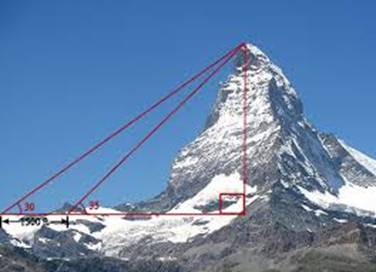
\includegraphics[scale=0.65]{"images/image018.jpg"}
\caption{ಟ್ರಿಗನಮಿಟ್ರಿಕಲ್​ ಸರ್ವೇಯಲ್ಲಿ ಪರ್ವತಗಳ ಎತ್ತರ}\label{art14-fig1}
\end{figure}

ಕರ್ನಲ್​ ವಾಗ್​ರವರ ಅಧಿಕಾರ ಅವಧಿಯಲ್ಲಿ, ನಾರ್ಥ್ ಈಸ್ಟರ್ನ್ ಸರಣಿಯ ಜೊತೆಗೆ ಕಾಶ್ಮೀರ ಪ್ರದೇಶ, ಪಂಜಾಬಿನ ಸಿಂಧ್​ ಪ್ರಾಂತ್ಯ ಈ ಪ್ರದೇಶಗಳಲ್ಲೂ ಸಹ ಟ್ರೈಯಾಂಗ್ಯುಲೇಷನ್​ ಕಾರ್ಯವನ್ನು ಭರದಿಂದ ವಿಸ್ತರಿಸಲಾಯಿತು. ಈ ಕಾಲಾವಧಿಯಲ್ಲಿ, ಇಡೀ ವಿಶ್ವದಲ್ಲಿ ಟ್ರೈಯಾಂಗ್ಯುಲೇಷನ್​ ಸರ್ವೇ ಕಾರ್ಯಕ್ಕೊಳಗಾದ ಒಟ್ಟು ಪ್ರದೇಶದ ನಾಲ್ಕನೇ ಒಂದು ಭಾಗ ಭಾರತದ ಒಳಗಡೆಯೇ ಆಗಿತ್ತು. ಇದುವರೆಗೆ ಯಾವುದೇ ಒಂದು ಸಂಸ್ಥೆ ಕೈಗೊಂಡ ಸರ್ವೇಗಳ ಪೈಕಿ ಭಾರತೀಯ ಈ ಸರ್ವೇಯೇ ಅತ್ಯಂತ ದೊಡ್ಡ ಸರ್ವೇ ಆಗಿದ್ದು ಒಂದು ದಾಖಲೆ.

\vskip 4pt

ಕಠಿಣ ಮಾರಕ ಹವೆಯಲ್ಲಿ, ಈ ನಾರ್ಥ್ ಈಸ್ಟರ್ನ್ ಸರಣಿಯ ಟ್ರೈಯಾಂಗ್ಯುಲೇಷನ್​ ಮಹಾಕಾರ್ಯವನ್ನು ಮಾಡಲಾಯಿತು. ನೂರಾರು ಬ್ರಿಟಿಷ್​ ಹಾಗೂ ಭಾರತೀಯ ಸರ್ವೇಯರುಗಳು ಒಂದೇ ಋತುವಿನಲ್ಲಿ, ಈ ನಾರ್ಥ್ ಈಸ್ಟರ್ನ್ ಸರಣಿ ಕಾರ್ಯಚರಣೆಯಲ್ಲಿ ಮಾರಕ ಹವೆಯಿಂದ ಮಡಿಯುತ್ತಾರೆ. ರಾಯಲ್​ ಜೀಯೋಗ್ರಫಿಕಲ್​ ಸೊಸೈಟಿಯ ಕ್ಲೆಮೆಂಟ್​ ಮಾರ್ಕಮ್ರವರು ಈ ದುರಂತಮಯ ಅವಘಡದ ಬಗ್ಗೆ ಬರೆಯುತ್ತಾರೆ: “ಸರ್ವೇಯರುಗಳ ಮರಣದಅ ಸಂಖ್ಯೆಯು, ದೊಡ್ಡ ಯುದ್ಧವೊಂದನ್ನು ಎದುರಿಸಿ ಮಡಿಯುವ ಯೋಧರ ಸಂಖ್ಯೆಗಿಂತಲೂ ಹೆಚ್ಚಾಗಿತ್ತು. ಆ ಮಾರಣಾಂತಿಕ, ವಿಷಮ ಹವೆಯಲ್ಲಿ, ನಾರ್ಥ್ ಈಸ್ಟರ್ನ್ ಸರಣಿ ಕಾರ್ಯಚರಣೆಯಲ್ಲಿ ತೊಡಗಿಸಿಕೊಂಡ ಸರ್ವೇರುಗಳ ಧೈರ್ಯವು, ಯುದ್ಧದಲ್ಲಿ ಹೋರಾಡುವ ಯೋಧರಿಗಿಂತಲೂ ಹೆಚ್ಚಿನದಾಗಿತ್ತು...”

\newpage

ಈ ನಾರ್ಥ್ ಈಸ್ಟರ್ನ್ ಸರಣಿಯನ್ನು \enginline{1845} ರಲ್ಲಿ ಆರಂಭಿಸಿ, \enginline{1850} ರಲ್ಲಿ ಮುಕ್ತಾಯಗೊಳಿಸಲಾಯಿತು. ಒಂದು ತುದಿಯಲ್ಲಿ ಉತ್ತರದ ಡೆಹರಾಡೂನ್​ ಬೇಸ್​ ಲೈನ್​. ಇನ್ನೊಂದು ತುದಿಯಲ್ಲಿ ಅಸ್ಸಾಂ ಸಮೀಪದ ಪೂರ್ನಿಯಾದ ಸೊನಕೊಡಾ ಬೇಸ್​ ಲೈನ್​. ಈ ಎರಡು ಬೇಸ್​ ಲೈನ್​ಗಳ ನಡುವಿನ, ನಾರ್ಥ್ ಈಸ್ಟರ್ನ್ ಸರಣಿಯ ಉದ್ದವು \enginline{1690} ಮೈಲುಗಳು. ಇದು ವಿಶ್ವದಲ್ಲಿಯೇ ಅತ್ಯಂತ ಉದ್ದವಾದ ಟ್ರೈಯಾಂಗ್ಯುಲೇಷನ್​ ಸರಣಿ ಎಂದು ಹೆಸರುವಾಸಿಯಾಗಿದೆ. ಈ ನಾರ್ಥ್ ಈಸ್ಟರ್ನ್ ಸರಣಿಯ ಸಹಾಯದಿಂದ ಹಿಮಾಲಯ ಪರ್ವತಗಳಅ ಶ್ರೇಣಿಯಲ್ಲಿನ ಉನ್ನತವಾದ \enginline{79} ವಿವಿಧ ಶಿಖರಗಳ ಎತ್ತರಗಳಅನ್ನು ನಿರ್ಧರಿಸಲು ಸಾಧ್ಯವಾಯಿತು.

